% Pedagogical slide deck for jiram_catalog.
% Companion to ../../PEDAGOGICAL_REVIEW.md; every slide footer cites the
% review section it corresponds to. metropolis is not installed on this
% system (checked with kpsewhich beamerthememetropolis.sty), so this
% deck uses the beamer "default" theme per the spec's fallback rule.
\documentclass[aspectratio=169,11pt]{beamer}

\usetheme{default}
\usecolortheme{seahorse}
\setbeamertemplate{navigation symbols}{}

\usepackage[utf8]{inputenc}
\usepackage[T1]{fontenc}
\usepackage{lmodern}
\usepackage{textcomp}
\usepackage{graphicx}
\usepackage{listings}
\usepackage{xcolor}
\usepackage{tikz}
\usetikzlibrary{arrows.meta,positioning,shapes.geometric,fit}
\usepackage{amsmath}
\usepackage{booktabs}

\definecolor{jirblue}{RGB}{40,70,120}
\definecolor{jirgold}{RGB}{180,120,20}
\definecolor{jirgray}{RGB}{90,90,90}
\setbeamercolor{structure}{fg=jirblue}
\setbeamercolor{title}{fg=jirblue}
\setbeamercolor{frametitle}{fg=jirblue}
\setbeamercolor{block title}{bg=jirblue!12,fg=jirblue}
\setbeamercolor{block body}{bg=jirblue!4}
\setbeamerfont{frametitle}{series=\bfseries}

\lstset{
  basicstyle=\ttfamily\scriptsize,
  breaklines=true,
  columns=fullflexible,
  keywordstyle=\color{jirblue}\bfseries,
  commentstyle=\color{jirgray}\itshape,
  stringstyle=\color{jirgold},
  showstringspaces=false,
  frame=single,
  rulecolor=\color{jirgray!40},
  backgroundcolor=\color{black!3}
}

% ---------------------------------------------------------------------
% Footer that cites the review section a slide corresponds to, rather
% than beamer's usual navigation dots. \revsec{X.Y} sets it per slide.
\newcommand{\currevsec}{}
\newcommand{\revsec}[1]{\gdef\currevsec{#1}}
\setbeamertemplate{footline}{%
  \leavevmode%
  \hbox{%
  \begin{beamercolorbox}[wd=.55\paperwidth,ht=2.6ex,dp=1.1ex,leftskip=.3cm]{author in head/foot}%
    \usebeamerfont{author in head/foot}\scriptsize jiram\_catalog: a pedagogical review
  \end{beamercolorbox}%
  \begin{beamercolorbox}[wd=.45\paperwidth,ht=2.6ex,dp=1.1ex,rightskip=.3cm plus1fil]{title in head/foot}%
    \usebeamerfont{title in head/foot}\scriptsize
    \ifx\currevsec\empty\else review \S\currevsec\ \textbullet\ \fi
    \insertframenumber\,/\,\inserttotalframenumber
  \end{beamercolorbox}}%
  \vskip0pt%
}

\title{\textbf{jiram\_catalog}}
\subtitle{A pedagogical review: two instruments, geometry, and scientific readiness}
\author{}
\date{\small Implementation through \texttt{1e2723d} --- 7 September 2026}

\begin{document}

\begin{frame}[plain]
  \titlepage
  {\small\color{jirgray} Companion to \texttt{PEDAGOGICAL\_REVIEW.md}; every footer cites the review section it expands on.}
\end{frame}

\begin{frame}{Outline}
  \revsec{}
  \tableofcontents
\end{frame}

% =======================================================================
\section{What the tool is for}
% =======================================================================

\begin{frame}{Juno JIRAM, in one slide}
  \revsec{1}
  \begin{itemize}
    \item Two-channel infrared camera on Juno: L-band (3.455~$\mu$m, aurora, H3$^+$) and M-band (4.780~$\mu$m, thermal, day \& night)
    \item Detector: 128 lines $\times$ 432 samples per band; 256-line \texttt{LM} products stack both bands, 10 gap lines removed
    \item Juno spins at 2~rpm (12~deg/s); JIRAM's despinning mirror holds one look steady per spin
    \item Initial JIRAM census: 85{,}108 archived camera frames (4 September build log); counts describe that snapshot
  \end{itemize}
  \vspace{0.3cm}
  \begin{block}{The archive's own labels do not tell you where a frame is pointed}
    They tell you which SPICE kernels were used to figure that out --- computing it yourself is the first half of this project.
  \end{block}
\end{frame}

% Refresh through 1e2723d.
\begin{frame}{JunoCam adds a different measurement}
  \revsec{1}
\begin{itemize}
    \item A spinning \textbf{pushframe camera}: an archived image contains successive 128$\times$1648 framelets, with physical filter strips
    \item Native RED, GREEN, BLUE and METHANE are instrument channels; RGB is a viewing composite
    \item Its unsigned detector samples and per-frame timing require a separate adapter, not JIRAM's float reader or single-frame epoch
    \item The common workspace starts after each instrument has explicit geometry, validity, units and source identity
  \end{itemize}
  \begin{block}{Current scope, 7 September 2026}
    Native JunoCam inspection is available. Failure exclusion and readiness checks decide which observations and calculations are accessible.
  \end{block}
\end{frame}

\begin{frame}{Repeat coverage determines the useful product}
  \revsec{1}
A small detector on a fast spacecraft gives two useful observing regimes. They describe \emph{measured overlap and timing}, not a permanent division of Jupiter.
  \vspace{0.4cm}
  \begin{columns}[T]
    \column{0.48\textwidth}
    \textbf{Repeated views of one patch}\\
    \small JIRAM polar campaigns motivate fixed-grid time stacks. Check the actual cadence and common valid area before treating them as motion data.
    \column{0.48\textwidth}
    \textbf{Individual mapped looks}\\
    \small Much of the available sampling motivates a strip library. A later visit can exist without a usable short-baseline sequence.
  \end{columns}
\end{frame}

\begin{frame}{Regime 1: polar / repeat-view}
  \revsec{1}
  \begin{itemize}
    \item Repeated observations: verify unique exposures, positive cadence and common footprint; polar location alone is insufficient
    \item Natural product: a \textbf{region time stack} --- every overlapping frame, reprojected onto one fixed grid, laid along a time axis
    \item Ground truth exists: Ingersoll et al.\ (2022, \emph{Nature Astronomy}), 48 archived PJ4 frames $\to$ 4 published polar mosaics + wind vectors
    \item Built by: \texttt{region-stack}, \texttt{movie}, \texttt{export-goflow}
  \end{itemize}
\end{frame}

\begin{frame}{Regime 2: a library of mapped looks}
  \revsec{1}
\begin{itemize}
    \item Useful even when a local sequence does not support motion retrieval
    \item Natural product: a \textbf{library} --- looks on local tangent-plane grids, queryable by latitude, epoch and illumination
    \item Intensity structure can be compared across appropriately grouped observations; this does not require pretending they are a movie
    \item JIRAM paths: \texttt{strips}, \texttt{strip-stats}; JunoCam has its own native image-to-strip adapter
  \end{itemize}
\end{frame}

\begin{frame}{The two regimes, side by side}
  \revsec{1}
\small
  \begin{tabular}{lll}
    \toprule
     & \textbf{repeated views} & \textbf{mapped-look library} \\
    \midrule
    product & region time stack & strip library \\
    grid & fixed per region & fixed per strip \\
    scientific question & change over a usable $\Delta t$ & spatial intensity structure \\
    evidence needed & cadence, navigation, shared mask & masks, units, resolution, grouping \\
    \bottomrule
  \end{tabular}\par
  \vspace{0.4cm}
  Published PJ4 JIRAM maps and vectors validate a particular campaign. They do not provide a mission-wide or JunoCam wind-accuracy guarantee.
\end{frame}

% =======================================================================
\section{Three archive facts}
% =======================================================================

\begin{frame}{Three JIRAM facts, found the hard way}
  \revsec{2}
  \begin{enumerate}
    \item Archive labels lose all geometry after orbit 38
    \item Image files are little-endian despite every label saying otherwise
    \item Sequence numbering is 1-based, and frame~1 never arrives
  \end{enumerate}
  \vspace{0.3cm}
  Each one is enforced today by a specific line of code, not a comment. Get any of them wrong and geometry corrupts silently.
\end{frame}

\begin{frame}{Fact 1: labels lose geometry after orbit 38}
  \revsec{2.1}
  \begin{quote}\small
    ``label geometry is ABSENT for orbits $\geq$ 39 ... and for most 256-line dual-band products ... 64{,}139/85{,}108 frames have no label centre.'' \\
    \hfill---\texttt{docs/build\_log\_2026-09-04.md}, step 3d/3e
  \end{quote}
  75\% of that JIRAM census has no usable label geometry at all.
\end{frame}

\begin{frame}{Fact 1: what it forced}
  \revsec{2.1}
  \begin{itemize}
    \item Label geometry could never be the foundation --- only a spot-check
    \item \texttt{geometry.py} + \texttt{geo.py} $\to$ \texttt{frames\_geo.parquet} became \textbf{mandatory} infrastructure, not a convenience
    \item Every downstream module reads \texttt{frames\_with\_geo()}; none fall back to label geometry, because for 3 in 4 frames there is nothing to fall back to
  \end{itemize}
\end{frame}

\begin{frame}{Fact 2: little-endian, despite every label}
  \revsec{2.2}
  The JIRAM labels declare \texttt{IEEE754MSBSingle} / \texttt{IEEE\_REAL} --- big-endian, unambiguously.
  \vspace{0.2cm}
  \begin{columns}
    \column{0.5\textwidth}
    \textbf{Read big-endian:}\\
    \small spans $-2.6\times10^{38}$ to $3.1\times10^{38}$, 143 NaNs
    \column{0.5\textwidth}
    \textbf{Read little-endian:}\\
    \small spans $-0.00017$ to $0.5547$ W~m$^{-2}$~sr$^{-1}$~$\mu$m$^{-1}$ --- matches the published map's $0.0060$--$0.5545$
  \end{columns}
  \vspace{0.3cm}
  Found independently twice, from two unrelated questions, both times by checking whether the numbers were physically plausible.
\end{frame}

\begin{frame}{Fact 2: what it forced}
  \revsec{2.2}
  \begin{itemize}
    \item JIRAM RDR raw-pixel reads use \texttt{'<f4'} --- the empirically verified type
    \item This rule is instrument-specific: JunoCam RDR uses \texttt{>u2}; EDR uses unsigned 8-bit counts (section 4.18)
    \item The original crawl-index spec still says ``big-endian'' --- explicitly superseded, left as historical record
  \end{itemize}
  \vspace{0.3cm}
  \textbf{Rule of this repo:} where code and an old spec disagree, the code wins, and the spec stays as a record of what was believed at the time.
\end{frame}

\begin{frame}{Fact 3: frame 1 never arrives}
  \revsec{2.3}
  \begin{quote}\small\raggedright
    ``sequence\_number is 1-based and frame 1 is never delivered (\texttt{seq\_n = sequence\_samples-1} always).'' \\
    \hfill---\texttt{docs/build\_log\_2026-09-04.md}, ``Facts'' after step 3d
  \end{quote}
  Exact in the reconstructed JIRAM census: delivered sequences omit their first commanded frame. JunoCam has a different image/framelet identity model.
\end{frame}

\begin{frame}[fragile]{Fact 3: what it forced}
  \revsec{2.3}
  \texttt{sequence\_number} cannot be trusted across a real gap either. \texttt{index.assign\_sequences} instead detects boundaries from observed behaviour:
\begin{lstlisting}[language=Python]
new sequence starts when:
    gap since previous frame > 45 s     # one spin ~30.5 s
 or sequence_number fails to increase
\end{lstlisting}
  Later JIRAM grouping (strip chunking, trackability pairing) trusts this reconstruction. Do not apply its 45-second rule to JunoCam framelets.
\end{frame}

% =======================================================================
\section{Architecture}
% =======================================================================

\begin{frame}{Layers, in build order}
  \revsec{3}
  \small
  \begin{enumerate}
    \item \texttt{pds.py} + \texttt{mirror.py} --- crawl and download the archive
    \item \texttt{labels.py} + \texttt{index.py} --- parse labels, build \texttt{frames.parquet}
    \item \texttt{geometry.py} + \texttt{kernels.py} --- the SPICE engine
    \item \texttt{geo.py} --- geometry for every frame $\to$ \texttt{frames\_geo.parquet}
    \item \texttt{vicar.py} + \texttt{reproject.py} --- ground-truth I/O, map grids, inverse camera
    \item \texttt{regions.py} $\to$ \texttt{stacks.py} / \texttt{strips.py} --- the two regimes
    \item \texttt{movie.py}, \texttt{export\_goflow.py}, \texttt{stats2d.py}, \texttt{trackability.py} --- exports and analysis
    \item \texttt{tracking.py} --- the standing acceptance test, not a pipeline stage
    \item \texttt{api/} + \texttt{frontend/} --- browsing and orchestration; \texttt{science.py} supplies analysis preparation and \texttt{api/science.py} the research endpoints
  \end{enumerate}
\end{frame}

\begin{frame}[fragile]{One frame's path: archive to product}
  \revsec{3.2}
  \begin{center}
\begin{lstlisting}[basicstyle=\ttfamily\tiny,frame=none]
JIRAM PDS archive --(pds.py, mirror.py)--> mirrored .LBL/.IMG
      --(labels.py, index.py)--> frames.parquet (+ sequences)
      --(geometry.py, geo.py)--> frames_geo.parquet
      |
      +-- regime 1: select_frames -> reproject_frame -> region stack .nc
      |        -> composite_sequences / movie.py / export_goflow.py
      +-- regime 2: unit_rows -> chunk_table -> build_strip -> strip .nc
      |        -> stats2d.strip_statistics -> stats NetCDF
      |
      +-- GUI: browse + science API -> gui_cache/research/, exports/
\end{lstlisting}
  \end{center}
\end{frame}

% Refresh through 1e2723d.
\begin{frame}{A second adapter, shared scientific contracts}
  \revsec{3.2}
\begin{center}
  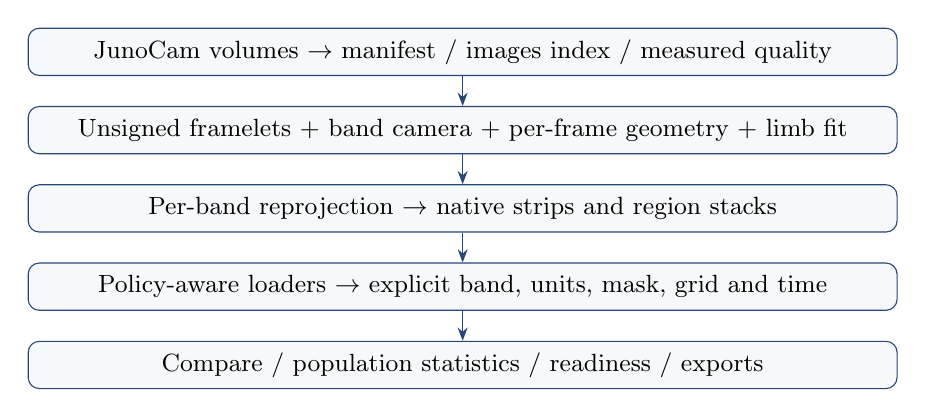
\begin{tikzpicture}[node distance=0.38cm, every node/.style={font=\small},
    box/.style={draw=jirblue,rounded corners,fill=jirblue!4,text width=10.8cm,align=center,minimum height=.60cm}]
    \node[box] (a) {JunoCam volumes $\to$ manifest / images index / measured quality};
    \node[box,below=of a] (b) {Unsigned framelets + band camera + per-frame geometry + limb fit};
    \node[box,below=of b] (c) {Per-band reprojection $\to$ native strips and region stacks};
    \node[box,below=of c] (d) {Policy-aware loaders $\to$ explicit band, units, mask, grid and time};
    \node[box,below=of d] (e) {Compare / population statistics / readiness / exports};
    \foreach \a/\b in {a/b,b/c,c/d,d/e} \draw[-{Stealth},jirblue] (\a)--(\b);
  \end{tikzpicture}
  \end{center}
\end{frame}

\begin{frame}{Where every product lives on disk}
  \revsec{3.3}
  \scriptsize
  \begin{tabular}{ll}
    \toprule
    product & path (relative to mirror root) \\
    \midrule
    label index & \texttt{index/frames.parquet} \\
    SPICE geometry & \texttt{index/frames\_geo.parquet} \\
    SPICE kernels & \texttt{spice/\{lsk,pck,fk,ik,sclk,spk,ck\}/} \\
    region stacks & \texttt{regions/<region>/<band>\_orbits<spec>\_<level>.nc} \\
    goflow realizations & \texttt{regions/<region>/goflow\_<band>\_orbits<spec>/rNNNNN/} \\
    strip NetCDFs \& index & \texttt{strips/orbitNN/<strip\_id>.nc}, \texttt{strips/strips.parquet} \\
    strip statistics & \texttt{strips/stats/} or \texttt{gui\_cache/stats\_<id>.nc} \\
    GUI cache/exports & \texttt{gui\_cache/}, \texttt{gui\_cache/exports/} \\
    \bottomrule
  \end{tabular}\par
\end{frame}

% Refresh through 1e2723d.
\begin{frame}{JunoCam and research paths stay separate}
  \revsec{3.3}
\small All paths below are relative to the mirror root.
  \vspace{0.2cm}
  \begin{tabular}{ll}
    \toprule
    product family & location \\
    \midrule
    archive manifest / every-version manifest & \texttt{junocam/manifest/} \\
    image, geometry and quality indexes & \texttt{junocam/index/} \\
    geometry and limb-fit cache & \texttt{junocam/geometry\_cache/} \\
    native region stacks & \texttt{regions/<region>/junocam\_*.nc} \\
    native strip products & \texttt{strips/junocam/orbitNN/} \\
    bounded PDS reference audit & \texttt{junocam/calibration\_review/} \\
    new research caches and movies & \texttt{gui\_cache/research/} \\
    browser velocity-model exports & \texttt{gui\_cache/exports/} \\
    \bottomrule
  \end{tabular}\par
  \vspace{0.3cm}
  Source files are preserved. Export destinations include the selected sources and settings; a changed policy cannot reuse stale realizations as a new result.
\end{frame}

% =======================================================================
\section{Deep dives}
% =======================================================================

\begin{frame}{Deep dives: what each one covers}
  \revsec{4}
  For every module: purpose, key data structures, the algorithm, what a modifier must know, the validation gate, and the scars.
  \vspace{0.3cm}

  19 teaching sections; the original JIRAM deep dives retain their numbers:
  \begin{itemize}
    \item archive mirror \& index (4.1--4.3)
    \item geometry \& kernels (4.4--4.6)
    \item map machinery \& regions (4.7--4.9)
    \item the two regimes (4.10--4.11, 4.13)
    \item validation \& analysis (4.12, 4.14--4.15)
    \item the GUI, config (4.16--4.17)
    \item JunoCam adapter and shared scientific workflow (4.18--4.19)
  \end{itemize}
\end{frame}

\begin{frame}{\texttt{pds.py} + \texttt{mirror.py}: archive mirror}
  \revsec{4.1}
  \textbf{Purpose:} Apache listings $\to$ manifest $\to$ verified download.
  \begin{itemize}
    \item Only the \texttt{Wget} user agent is permitted under \texttt{/PDS/}; every download is a real \texttt{wget} subprocess
    \item Completeness = exact declared byte count from the sibling label, or last line \texttt{END}, or trailing \texttt{</Product\_Observational>}
    \item \texttt{--verify} re-checks MD5 and re-downloads mismatches once
  \end{itemize}
  \textbf{Scar:} orbit50's listing alone is $\sim$36~MB HTML --- large enough to need retry-with-backoff, not a single timeout.
\end{frame}

\begin{frame}{\texttt{labels.py}: PDS3 parsing}
  \revsec{4.2}
  \textbf{Purpose:} one \texttt{.LBL} $\to$ one flat, typed dict --- tolerantly.
  \begin{itemize}
    \item \texttt{pvl.load}, then a fallback grammar, then require the last line to be literally \texttt{END}
    \item A parse failure never raises: the row still exists, \texttt{parse\_ok=False}, every geometry column NaN
    \item \texttt{"N/A"} (any case) is the \emph{only} missing-value sentinel the archive uses
    \item \texttt{geom\_band}: whichever band group has a numeric \texttt{CENTER\_LATITUDE} --- independent of which band the image data actually is
  \end{itemize}
\end{frame}

\begin{frame}{\texttt{index.py}: sequence segmentation}
  \revsec{4.3}
  \textbf{Purpose:} multiprocess label parse $\to$ \texttt{frames.parquet}, then segment sequences over the \emph{whole} sorted table.
  \begin{itemize}
    \item \texttt{orbit} is float64 (4{,}697 nulls); \textbf{always use \texttt{orbit\_dir}}, never \texttt{orbit}
    \item \texttt{orbit} disagrees with \texttt{orbit\_dir} on 3{,}900 rows --- all \texttt{orbit03}, labelled \texttt{ORBIT\_NUMBER=1}; an archive property, not a bug
    \item sequence columns are recomputed over the combined table every run, never patched incrementally
  \end{itemize}
\end{frame}

\begin{frame}[fragile]{\texttt{geometry.py}: the pinhole model}
  \revsec{4.4}
  \textbf{Purpose:} per pixel, per frame $\to$ lat/lon/range/emission/incidence/phase, no per-pixel Python loop.
\begin{lstlisting}[language=Python]
x = ifov * (lines/2 + 0.5 - line)      # 1-based line index
y = ifov * (samples/2 + 0.5 - sample)  # 1-based sample index
d = (x, y, 1) / |(x, y, 1)|            # unit ray, band frame
\end{lstlisting}
  One vectorised numpy op over the whole \texttt{(lines, samples, 3)} grid --- never per pixel. Then \texttt{pxform}: band frame $\to$ \texttt{J2000} $\to$ \texttt{IAU\_JUPITER}.
\end{frame}

\begin{frame}{\texttt{geometry.py}: the aberration fix}
  \revsec{4.4}
  \texttt{sincpt}'s \texttt{srfvec} and every pixel ray are \emph{apparent} (light-time + stellar aberration). Both must be un-aberrated \emph{the same way} before the ellipsoid intercept.
  \vspace{0.2cm}
  \begin{block}{Original spec: un-aberrate rays only}
    per-pixel error vs. oracle: \textbf{4e-3 deg}
  \end{block}
  \begin{block}{Corrected: un-aberrate \texttt{srfvec} too}
    per-pixel error vs. oracle: \textbf{8e-5 deg} --- a 50$\times$ reduction
  \end{block}
  Order of the mistake: $|v|/c \approx$ 7 arcsec $\approx$ 4~km on Jupiter's surface at perijove range.
\end{frame}

\begin{frame}{\texttt{geometry.py}: epoch sensitivity \& mirror-blind}
  \revsec{4.4}
  \begin{itemize}
    \item Juno spins at 12~deg/s: a 0.1~s epoch error moves the boresight $>1$~deg
    \item For this JIRAM geometry model, use the label's \texttt{START\_TIME}; the tested mid-exposure alternative was off by \emph{tens of degrees}
    \item Engine is deliberately \textbf{mirror-blind}: models bus attitude only, not JIRAM's despinning mirror
  \end{itemize}
  \vspace{0.2cm}
  Validated before writing code: mirror-blind SPICE matched 48 label centres to median 0.006~deg lat/lon, 0.017~deg emission, 28~km altitude.
\end{frame}

\begin{frame}{\texttt{kernels.py}: SPICE kernel management}
  \revsec{4.5}
  \begin{itemize}
    \item Static set (leap-seconds, planetary constants, one frame/instrument kernel) + per-orbit CK/SPK named in the labels
    \item Operational server first, PDS SPICE archive as fallback (renames SPKs: \texttt{spk\_rec\_*} $\leftrightarrow$ \texttt{juno\_rec\_*})
    \item \texttt{naif.jpl.nasa.gov} fails system-CA TLS; every fetch pinned to the \texttt{certifi} bundle
  \end{itemize}
  \textbf{Open kernel coverage:} the earlier six long CK gaps did not explain every failure. Orbits 38/55 lack attitude coverage; orbit 70 lacks trajectory coverage. The missing intervals remain unresolved.
\end{frame}

\begin{frame}{\texttt{geo.py}: augmenting every frame}
  \revsec{4.6}
  \begin{itemize}
    \item \texttt{spawn} workers (never \texttt{fork}) --- SPICE kernel pool is per-process global state
    \item One row per (frame, band half); a 256-line \texttt{LM} product $\to$ 2 rows
    \item A frame's computation failure never aborts the run: \texttt{geo\_ok=False}, error text recorded, row still exists
  \end{itemize}
\end{frame}

\begin{frame}{\texttt{geo.py}: the label-centroid caveat}
  \revsec{4.6}
  \begin{alertblock}{\texttt{bore\_lat} $\neq$ label \texttt{CENTER\_LATITUDE} for a partial frame}
    \texttt{bore\_lat}: the boresight's own intercept, NaN if the boresight misses. \\
    Label centre: a \emph{visible-area centroid} for a partial (limb) frame.
  \end{alertblock}
  Comparing the two without filtering to fully-on-planet frames looks like a large geometric error that is really just two different definitions of ``centre.''
  \vspace{0.2cm}
  \textbf{Open:} L-band residual (median 0.024~deg) is roughly double M-band's (0.010~deg) --- both inside the M-only gate tolerance; cause unresolved.
\end{frame}

\begin{frame}{\texttt{vicar.py}: reading the ground truth}
  \revsec{4.7}
  \begin{itemize}
    \item JPL's older format: ASCII label \emph{inside} the file, not a sidecar
    \item Label size (\texttt{LBLSIZE}) always read from the file, never hard-coded --- the paper's own supplementary readers hard-code 12{,}800 bytes and silently misparse the 1{,}728-byte \texttt{.tp4} vector tables
    \item \texttt{EOL=1}: a \emph{second} trailing label after the data (TRACKER4's own processing history)
  \end{itemize}
\end{frame}

\begin{frame}[fragile]{\texttt{reproject.py}: the inverse camera model}
  \revsec{4.8}
  \texttt{project\_to\_pixels}: run \texttt{geometry.py}'s chain backwards.
\begin{lstlisting}[basicstyle=\ttfamily\tiny,frame=none]
(lat,lon) -> surface point -> IAU_JUPITER -> J2000
   -> re-apply FORWARD stellar aberration (put it back!)
   -> band frame -> invert pinhole -> fractional (line, sample)
\end{lstlisting}
  Round-trip residual on a live frame: \textbf{1.22e-05 px}. \\
  \texttt{reproject\_frame}: walk the \emph{output} grid, pull from the source --- no output pixel unpainted, no input pixel double-scattered.
\end{frame}

\begin{frame}{\texttt{reproject.py}: stereographic was wrong}
  \revsec{4.8}
  \small
  \begin{tabular}{lrrr}
    \toprule
    candidate & centroid RMS (px) & sing.\ ratio & km/px \\
    \midrule
    stereographic & 0.828 & 1.00178 & 15.069 \\
    \textbf{orthographic (ellipsoid)} & \textbf{0.339} & \textbf{1.00010} & \textbf{15.005} \\
    \bottomrule
  \end{tabular}\par
  \vspace{0.3cm}

  Every JIRAM paper checked calls the polar maps ``stereographic.'' The fit says otherwise, decisively: the map \emph{is} the body-fixed equatorial plane, orthographically projected --- no trig at all once you have the 3-D point.
\end{frame}

\begin{frame}{\texttt{reproject.py}: the radius degeneracy}
  \revsec{4.8}
  Three candidate radii (polar, equatorial, $\sqrt{ac}$) were proposed for the fit.
  \begin{alertblock}{They cannot be distinguished by residual at all}
    $\rho \propto R$ for every radial law --- registration only ever measures the \emph{ratio} $R / \text{km\_per\_px}$, never $R$ alone.
  \end{alertblock}
  Settled instead by requiring self-consistency with the one independently stated number: the label's own \texttt{MPS=15.0}.
\end{frame}

\begin{frame}{\texttt{regions.py}: two grid rules}
  \revsec{4.9}
  \begin{itemize}
    \item \texttt{polar\_ortho}: the published rule, generalised to either pole, any central meridian --- \texttt{north\_pole\_paper} reproduces \texttt{PAPER\_GRID} exactly
    \item \texttt{local\_ortho}: tangent plane at an arbitrary centre, dropped onto the ellipsoid along the local normal --- every mid-latitude strip's grid
  \end{itemize}
  \vspace{0.2cm}
  A new named region (e.g.\ the Great Red Spot) is a \textbf{4-line YAML addition}, no code.
\end{frame}

\begin{frame}{\texttt{regions.py}: the visibility subtlety}
  \revsec{4.9}
  Naive test $(P-c)\cdot up > 0$ fails: the tangent plane touches the ellipsoid \emph{only} at $c$, so this is $\leq 0$ almost everywhere --- near side and far side alike.
  \begin{block}{Correct test: use the surface normal at $P$ itself}
    $\text{visible} = \big(\text{normal}(P)\cdot up\big) > -\text{tol}$
  \end{block}
  Exactly the silhouette condition a rendering engineer would recognise.
\end{frame}

\begin{frame}{\texttt{stacks.py}: selection, three cost tiers}
  \revsec{4.10}
  \texttt{select\_frames}, cheapest test first:
  \begin{enumerate}
    \item Scalar quality cuts on \texttt{frames\_geo.parquet} --- free
    \item Bounding-box prefilter against the region --- free, approximate
    \item Exact test: fresh geometry, every 4th pixel, must land on canvas --- expensive, exact
  \end{enumerate}
  Three tiers, three cost levels, cheapest first --- run the expensive exact test only on what already survived the free filters.
\end{frame}

\begin{frame}{\texttt{stacks.py}: memory design}
  \revsec{4.10}
  \begin{itemize}
    \item One geometry-only pass unions every frame's footprint box \emph{before} any pixel is reprojected
    \item Output array allocated \textbf{once}, at the tight window's size --- never at the full region canvas (a \texttt{north\_pole} region is 3600$\times$3600)
    \item \texttt{spawn} workers each return only their own frame's footprint box, not the shared window
  \end{itemize}
  Initial JIRAM PJ4 measurement: 294 frame steps, 2.25~GB. Sequence composite: 25 steps, more valid coverage than any one frame.
\end{frame}

\begin{frame}{\texttt{movie.py} + \texttt{export\_goflow.py}}
  \revsec{4.11}
  \begin{itemize}
    \item \textbf{One whole-stack} brightness stretch, not per-frame --- a per-frame stretch would \emph{hide} the wobble that reveals a bad reprojection
    \item \texttt{export\_goflow}: cuts variable-cadence stacks into constant-cadence \emph{runs}; invalid pixels \textbf{zero-encoded} (not NaN) to match the downstream model's own convention
    \item No \texttt{u\_mid}/\texttt{v\_mid}: real data has no ground-truth velocity, unlike the synthetic sets this layout was designed to match
  \end{itemize}
\end{frame}

\begin{frame}{\texttt{tracking.py}: masked NCC as cost volumes}
  \revsec{4.12}
  90\% of a published map is exact-zero background; validity has to be a first-class concept, and the mask \emph{depends on trial displacement}.
  \vspace{0.2cm}
  6 masked window sums $\times$ 1225 trial displacements per template --- one at a time is hopeless.
  \begin{block}{Cost volumes}
    Each sum, at one fixed displacement, is a box filter over the whole tile --- serves every template in that tile at once.
  \end{block}
  Measured throughput: \textbf{2{,}141 templates/s} on one core.
\end{frame}

\begin{frame}{\texttt{tracking.py}: the reversed line axis}
  \revsec{4.12}
  \small
  \begin{tabular}{lrr}
    \toprule
    line axis & centre-on-footprint & full-template-on-footprint \\
    \midrule
    direct & 0.0\% & 0.0\% \\
    reversed & 96.4\% & 91.4\% \\
    \bottomrule
  \end{tabular}\par
  \vspace{0.3cm}

  \texttt{row = NL - 1 - (line - 1)} --- settled unambiguously by footprint overlap. \\
  0-vs-1-based index origin: genuinely underdetermined --- the two conventions differ by 0.0005~px in the pooled result, ``the tracking cannot separate them, which is the point.''
\end{frame}

\begin{frame}{\texttt{tracking.py}: the gate numbers}
  \revsec{4.12}
  \small
  \begin{tabular}{lrrr}
    \toprule
     & n & median (px) & frac $<1$px \\
    \midrule
    A: paper maps vs.\ TRACKER4 & 516{,}517 & 0.224 & 83.4\% \\
    B: our reprojections vs.\ TRACKER4 & 515{,}377 & 0.434 & 80.1\% \\
    \bottomrule
  \end{tabular}\par
  \vspace{0.3cm}

  The A$\to$B gap ($\sim$0.2~px) is the honest cost of the full geometry+reprojection chain, on top of the tracker's own noise floor.
  \vspace{0.2cm}
  \textbf{Scar:} 2 of 24 pairs (\texttt{n0204aa/bb}) sit near 1.04~px median --- pooled statistic absorbs it, per-pair table reveals it.
\end{frame}

\begin{frame}{\texttt{strips.py}: chunking a sequence}
  \revsec{4.13}
  A single commanded sequence can slew tens of degrees while it runs. A chunk ends when:
  \begin{itemize}
    \item great-circle distance from the \emph{chunk's first row} exceeds 12~deg, \emph{or}
    \item the time gap exceeds 120~s
  \end{itemize}
  Chunks under \texttt{min\_frames} are dropped but still consume a \texttt{chunk\_index} --- so a strip's name never shifts if the threshold changes later.
\end{frame}

\begin{frame}{\texttt{strips.py}: resolution classes}
  \revsec{4.13}
  \texttt{RESOLUTION\_CLASSES} = (2, 3, 5, 7, 10, 15, 20, 30, 50, 70, 100, 150, 200, 300)~km/px --- log-nearest snap, ties to the finer class.
  \vspace{0.2cm}
  \begin{block}{Why quantise at all}
    Two strips of the same class compare spectrum-to-spectrum, structure-function-to-structure-function, \textbf{with no resampling} --- resampling would contaminate exactly the small-scale statistics being measured.
  \end{block}
  Initial JIRAM result: 289 strips, orbits 4+24, both bands, 392~MB. This is a historical build measurement, not the current mixed-instrument count.
\end{frame}

\begin{frame}{\texttt{stats2d.py}: the recipe}
  \revsec{4.14}
  Every diagnostic in this module follows one recipe, because a strip is a field with holes:
  \begin{enumerate}
    \item detrend over \emph{valid} pixels only
    \item fill invalid pixels with that same mean
    \item taper the whole canvas (Tukey/Hann)
    \item divide by $\text{valid\_frac} \times \text{window\_power}$
  \end{enumerate}
  Result: a fully-valid, untapered field obeys Parseval exactly; a masked field is unbiased in \emph{total} variance to first order.
\end{frame}

\begin{frame}{\texttt{stats2d.py}: mask leakage --- stated, not fixed}
  \revsec{4.14}
  Masking \emph{convolves} the true spectrum with the mask's own spectrum --- moves variance across $k$ even when the total is right.
  \begin{itemize}
    \item Smooth, sparse holes: mild distortion. Measured: slope $-2.97$ unmasked vs.\ $-2.92$ with 15\% masked
    \item Speckle masks: broadband leakage --- \textbf{``no scalar correction can repair''} this (module's own words)
  \end{itemize}
  A documented, \emph{measured} limitation, not hidden and not over-corrected.
\end{frame}

\begin{frame}{\texttt{stats2d.py}: bicoherence}
  \revsec{4.14}
  $b^2 = \dfrac{|\sum_s X_s(k_1)X_s(k_2)X_s^*(k_1{+}k_2)|^2}{\sum_s|X_s(k_1)X_s(k_2)|^2 \cdot \sum_s|X_s(k_1{+}k_2)|^2} \in [0,1]$
  \vspace{0.2cm}

  1.0 when the sum-mode phase is \emph{locked} to the two parents' phases every segment; falls toward $1/n_{\text{segments}}$ when random.
  \vspace{0.2cm}
  Test: same power spectrum, coupled vs.\ independent third-term phase $\to$ $b^2 > 0.5$ vs.\ $b^2 < 0.1$ at the same bin --- detects coupling an ordinary spectrum cannot see at all.
\end{frame}

\begin{frame}{\texttt{trackability.py}: before any pixel is reprojected}
  \revsec{4.15}
  Pure numpy/pandas, no SPICE, no imagery. Candidate pair: same orbit/band, 90~s--6~h apart, boresights within a generous separation proxy.
  \begin{alertblock}{The threshold alone over-admits}
    Dense polar mosaics: one boresight falls near \emph{several} raster positions in the next sequence, not just its true repeat --- verified numerically (closest wrong-position pair $<$ farthest correct-position pair).
  \end{alertblock}
  Fix: keep only the \textbf{nearest partner per sequence} --- on top of the threshold, not instead of it.
\end{frame}

\begin{frame}{\texttt{trackability.py}: the best-baseline redefinition}
  \revsec{4.15}
  \begin{columns}
    \column{0.48\textwidth}
    \textbf{Original:} partner whose displacement is closest to 5~px
    \column{0.48\textwidth}
    \textbf{Revised:} smallest $dt$ among \emph{trackable} partners
  \end{columns}
  \vspace{0.3cm}
  A sequence hours away could \emph{coincidentally} land closer to 5~px than the true nearest repeat and win. ``Smallest usable $dt$'' has no such failure mode.
  \vspace{0.2cm}
  Initial JIRAM totals: 29{,}862 unit frames, 16{,}541 with a partner, 7{,}493 trackable at 30~m/s, 61 orbits. JunoCam trackability remains unassessed by this model.
\end{frame}

\begin{frame}{Five views follow five scientific tasks}
  \revsec{4.16}
\small
  \begin{tabular}{lp{9.8cm}}
    \toprule
    \textbf{Explore} & Find observations; inspect identity, footprint, date and band. \\
    \textbf{Time series} & Inspect a fixed-grid stack; check cadence and export readiness. \\
    \textbf{Image library} & Inspect strips; request individual or population statistics. \\
    \textbf{Compare} & Align the view, blink sources and inspect registration diagnostics. \\
    \textbf{Coverage} & Distinguish archive-known, local, navigated and eligible products. \\
    \bottomrule
  \end{tabular}\par
  \vspace{0.3cm}
  One \texttt{zustand} store and typed Arrow arrays connect the views. Legacy internal identifiers \texttt{catalog/poles/strips} remain for compatibility; the labels now describe tasks.
\end{frame}

\begin{frame}{Leave room for the image, then reveal detail}
  \revsec{4.16}
\begin{itemize}
    \item Explore starts with \textbf{coverage density}; swath outlines, coordinate conventions and selected footprints can be inspected explicitly
    \item A collapsible selection tray and metadata panels protect image area; controls wrap and statistics panels keep a usable minimum height
    \item Grayscale PNG stores value in R and validity in alpha; local colour-map lookup changes appearance without a new scientific calculation
    \item Orthographic navigation uses a scalar zoom, preserving aspect ratio; RGB uses a separate composite path
  \end{itemize}
\end{frame}

\begin{frame}{A selection should say what the next action means}
  \revsec{4.16}
\begin{itemize}
    \item Stable product/half keys survive reordering; metadata shows version identity and quality reasons
    \item ``Browse images from these orbits'' transfers an \emph{orbit filter}, not an exact claim that the listed strips contain every selected exposure
    \item Stack builds, movie renders and exports are jobs with visible progress; polling remains available during long work
    \item Coverage keeps excluded and unassessed JunoCam entries metadata-only, including direct thumbnail access
  \end{itemize}
  \begin{block}{Interaction is part of scientific provenance}
    The currently named source and settings must describe the pixels actually on screen.
  \end{block}
\end{frame}

% Refresh through 1e2723d.
\begin{frame}{A late response must not relabel old pixels}
  \revsec{4.16}
Suppose RED finishes loading after the user has already selected GREEN.
  \vspace{0.3cm}
  \begin{enumerate}
    \item Identify a request by source, frame, band/RGB, normalization, stretch, size and every other setting carried on the image request
    \item Clear previously displayed pixels while a new uncached request is pending; otherwise the new label describes the old image
    \item Accept completion only if its full request identity is still current
  \end{enumerate}
  \vspace{0.2cm}
  An out-of-order regression checks the race. A browser assertion must wait for actual visible pixels, not merely a changed control or an empty canvas.
\end{frame}

\begin{frame}{Responsive browsing does not change the estimator}
  \revsec{4.16}
\begin{itemize}
    \item Statistics start on request. A 6000$\times$6000 native JunoCam strip can take several minutes; the interface says so while it is pending
    \item Preview metadata slices \emph{before} loading array values; graticules and local-time contours use a bounded grid
    \item Display ranges share reads across normalization choices. Source signatures invalidate caches when inputs or policy change
    \item Native scientific normalization, FFTs and structure functions retain native pixels; no faster estimator was silently substituted
  \end{itemize}
\end{frame}

\begin{frame}{The NetCDF lock protects correctness, with a cost}
  \revsec{4.16}
\begin{itemize}
    \item Concurrent NetCDF reads caused a real process crash. A shared lock now spans complete image, coverage and science routes and relevant jobs
    \item An image request can queue behind requested native statistics; serialization does not make every operation instantly responsive
    \item Health, job status, configuration and Arrow catalog reads remain outside that lock
    \item Single-flight table caches avoid duplicate cold loads; Arrow uses an explicit bounded pool instead of inheriting a pathological one-thread setting
  \end{itemize}
  \vspace{0.2cm}
  Concurrency checks therefore verify both protected access and the independent status paths.
\end{frame}

\begin{frame}{\texttt{config.py} + the subcommand pattern}
  \revsec{4.17}
  \begin{itemize}
    \item Precedence: explicit arg $>$ env var $>$ TOML file $>$ built-in default --- resolved \emph{at call time}, never cached at import
    \item \texttt{add\_subparser(subparsers)} / \texttt{run(args)}: a module owns its own CLI surface; \texttt{cli.py} wires it in afterward
    \item Enforces a project rule: executors never edit \texttt{cli.py}, \texttt{pyproject.toml}, \texttt{uv.lock} directly --- exactly where concurrent milestones would collide
  \end{itemize}
\end{frame}

% Refresh: new review section 4.18.
\begin{frame}{JunoCam: identify the observation before counting it}
  \revsec{4.18}
\begin{itemize}
    \item \texttt{junocam/pds.py} discovers published volumes and builds an archive manifest; downloaded labels and images populate a separate local index
    \item A later \texttt{\_V02} release can supersede \texttt{\_V01}. They represent one observation, even if corrected label times differ by milliseconds
    \item Defaults select the \textbf{latest known version}, then require eligibility. They do not silently fall back to a clean older release
    \item An eligible older version can be inspected explicitly; derived products retain their stored source-version provenance
  \end{itemize}
  Archive discovery, local availability and scientific eligibility are three different counts.
\end{frame}

\begin{frame}{JunoCam: an image is a sequence of band framelets}
  \revsec{4.18}
\begin{block}{\texttt{junocam/images.py}: natural array shape}
    $(n_{\rm frames},\ n_{\rm bands},\ 128,\ 1648)$; bands cycle inside each frame in the label's \texttt{FILTER\_NAME} order.
  \end{block}
  \begin{itemize}
    \item RDR: unsigned big-endian 16-bit values (\texttt{>u2}), already linearized DN
    \item EDR: unsigned 8-bit companded counts; the SIS \texttt{SQROOT} lookup restores the linear count scale
    \item The table is not a fitted square-root formula: code 23 maps to 23, code 255 maps to 2879
    \item Shape and sample count are checked; summed products on a different detector grid are rejected
  \end{itemize}
\end{frame}

\begin{frame}{JunoCam: the camera is a band-dependent geometry}
  \revsec{4.18}
\begin{itemize}
    \item \texttt{camera.py} reads focal length, distortion centre and radial distortion from the instrument kernel
    \item Array indices refer to pixel centres; the kernel's framelet coordinates start at a corner. The $+0.5$ conversion is deliberate
    \item Different filters occupy different focal-plane strips. One ground feature crosses them in different frames as Juno spins
    \item Reprojection can bring those observations together only with the correct camera \emph{and} frame timing; a colour fringe is a diagnostic, not just a display defect
  \end{itemize}
\end{frame}

\begin{frame}{JunoCam: use an epoch for each frame}
  \revsec{4.18}
\small
  \[
    t_i = t_{\rm start}+b_{\rm start}
          + i\bigl(\Delta t_{\rm label}+\delta t_{\rm IK}\bigr)
          + \delta t_{\rm fitted} .
  \]
  \normalsize
  \begin{itemize}
    \item Commanded bands share a readout epoch within one frame; the next frame gets a new attitude and observer geometry
    \item \texttt{geometry.py} stores per-frame transformations for the inverse camera path
    \item \texttt{limb.py} fits one start-time offset per image against the predicted ellipsoid limb; it cannot absorb arbitrary frame-to-frame jitter or a wrong timing rate
  \end{itemize}
  At Juno's spin rate, millisecond timing errors can produce visible subpixel shifts.
\end{frame}

\begin{frame}{JunoCam: a limb fit is evidence with limits}
  \revsec{4.18}
\begin{enumerate}
    \item Interpolate the predicted ray/ellipsoid discriminant through zero: a smooth boundary avoids whole-row quantization
    \item Detect the observed edge, fit an offset, then detect and fit again; compare before/after residuals on the same final point set
    \item Inspect entering and leaving limbs separately. Haze above the reference ellipsoid can shift an apparent limb without a pointing error
  \end{enumerate}
  \vspace{0.2cm}
  The PJ4 assessment records limb-height and interframe-rate residuals. It retains the kernel timing rate; a low fitted residual does not establish independent navigation accuracy.
\end{frame}

\begin{frame}{JunoCam: reproject each band and preserve its support}
  \revsec{4.18}
\begin{itemize}
    \item \texttt{reproject.py} walks output cells through each frame's stored inverse transform, then bilinearly samples the appropriate filter strip
    \item Facing-surface, detector bounds and photoactive-column tests restrict valid contributions
    \item Per-band sums and hit counts produce a mean where observed and NaN where there is no support
    \item \texttt{stacks.py} and \texttt{strips.py} write fixed-grid products; masks, bands and source identities travel with the pixels
  \end{itemize}
  A displayed RGB composite is assembled from those physical bands; it is not a fifth measured channel.
\end{frame}

\begin{frame}{JunoCam: quality is an access decision with evidence}
  \revsec{4.18}
\small
  \begin{tabular}{lp{10cm}}
    \toprule
    \textbf{Excluded} & Documented affected images/intervals, measured signal failures or failed geometry; pixels withheld. \\
    \textbf{Unassessed} & Incomplete metrics or no affirmative unaffected-image evidence; pixels withheld. \\
    \textbf{Eligible} & Complete clean metrics and supported evidence under the versioned policy; navigation status remains explicit. \\
    \bottomrule
  \end{tabular}\par
  \vspace{0.3cm}
  \texttt{failure-exclusion-v1} keeps instrument, signal and navigation reasons distinct. A legacy A/B/C grade or ``post-anneal'' epoch does not establish recovery.
  \vspace{0.2cm}

  Loaders enforce this for images and derived analysis/export access. No browser override reveals withheld pixels.
\end{frame}

\begin{frame}{JunoCam: what the current eligible sample supports}
  \revsec{4.18}
\begin{itemize}
    \item At \texttt{1e2723d}: \textbf{72 preferred eligible PJ4 observations} in the current mirror
    \item Compared with the earlier 93 mapped observations, 21 methane observations are additionally withheld by existing bloom flags; no RGB observation is removed by this additional cut
    \item The bloom metric is conservative signal evidence, not proof of a documented hardware event in every flagged image
    \item The polar stack contains \textbf{three unique observations}; gaps are about 577 and 243 seconds, outside a 5\% constant-cadence tolerance
  \end{itemize}
  Viewing those three maps is useful. Calling them an export-ready regular three-frame sequence would be incorrect.
\end{frame}

\begin{frame}{PDS ``calibrated'' is a derived reference here}
  \revsec{4.18}
\begin{itemize}
    \item The ML collection preprocesses, flattens, reprojects and mosaics native inputs before generating Hubble-equivalent channels
    \item Its five channels include predicted UV and methane values; these are not five simultaneous native measurements
    \item Useful role: broad morphology and method comparison. Native motion, intensity spectra and cross-instrument radiometry require separate validation
    \item A plausible generated image does not establish repair of an instrument failure or make its damaged input eligible
  \end{itemize}
  Coverage links to the collection as a reference. No automatic native import or repaired-data certification is enabled.
\end{frame}

\begin{frame}{PDS reference: what the bounded audit actually measured}
  \revsec{4.18}
\small
  \begin{itemize}
    \item Inventory: 37{,}386 tile identifiers across PJ13--36; overlapping tiles are not that many independent exposures
    \item Three sampled PJ13 TIFFs: $256\times256\times5$, float32, 62.5~km grid spacing, LAEA with planetographic latitude
    \item All three labels have nil observation times. The sampled mosaic spans about 130 minutes; no per-pixel timing was established
    \item Actual FITS rows already contain values below 1; a guide's extra division by 255 would mis-scale them. Zeros and the labelled invalid sentinel require mask reconciliation
  \end{itemize}
  \vspace{0.1cm}
  \texttt{docs/reports/junocam\_calibrated\_assessment\_2026-09-07.md} records sources, hashes and limits. Three tiles plus headers/rows cannot certify the entire collection.
\end{frame}

% Refresh: new review section 4.19.
\begin{frame}{Choose the physical quantity before its colour scale}
  \revsec{4.19}
\begin{itemize}
    \item \texttt{science.py} selects one physical band, validates the grid, prepares native arrays and records provenance
    \item JIRAM measures spectral radiance; native JunoCam products here carry DN. An illumination transform does not turn DN into calibrated I/F
    \item RGB is accepted for viewing. Statistics, motion-model exports and physical-band movies require an actual available channel
    \item Brightness stretch maps values to display levels; scientific normalization changes the field whose statistics are calculated
  \end{itemize}
  A plot labelled by instrument, band, units and normalization names a reproducible quantity.
\end{frame}

\begin{frame}{Illumination correction has a domain of validity}
  \revsec{4.18}
For reflected light, write $\mu_0=\cos i$ and $\mu=\cos e$.
  \[
    I_{\rm Lambert}=I/\mu_0, \qquad
    I_{\rm Minnaert}=I/(\mu_0^k\,\mu^{k-1}).
  \]
  \begin{itemize}
    \item Incidence is required; Minnaert also requires emission. JunoCam masks incidence $\geq88^\circ$; cosine floors guard division near the limb/terminator
    \item These models reduce illumination trends; they do not establish absolute radiometry or preserve every spatial statistic
    \item JIRAM thermal radiance retains nightside emission. Reflected-light Lambert/Minnaert requests are rejected for it
  \end{itemize}
\end{frame}

\begin{frame}{The same smoothing number can mean a different scale}
  \revsec{4.18}
\texttt{flat:sigma} divides by a Gaussian low-pass background and normalizes the result. Sigma is expressed in \emph{the array's pixels}.
  \vspace{0.3cm}
  \begin{columns}[T]
    \column{0.48\textwidth}
    \textbf{Image preview}\\
    \small Operates after serving stride; sigma is in preview pixels. It is a viewing aid.
    \column{0.48\textwidth}
    \textbf{Analysis and export}\\
    \small Operates on native pixels before scientific calculations; the recipe records this choice.
  \end{columns}
  \vspace{0.4cm}
  If a preview keeps every fourth pixel, sigma 10 spans four times the physical distance of native sigma 10. Compare normalization groups using their recorded physical context.
\end{frame}

\begin{frame}{Readiness checks a sequence, not a wind result}
  \revsec{4.19}
\begin{enumerate}
    \item Deduplicate source versions; select a physical band and validate pixel scale and any supplied regular, square grid coordinates
    \item Require unique observations with strictly positive time gaps
    \item Find runs of at least three frames whose gaps satisfy the cadence tolerance
    \item Apply the selected normalization and require pixels valid in \emph{every} frame of a run
  \end{enumerate}
  \vspace{0.2cm}
  Report observation count, gaps, cadence runs and explicit failure reasons. A cadence run can contain several sliding triples; its count is not the number of all triples.
\end{frame}

\begin{frame}{An export carries the recipe that made its arrays}
  \revsec{4.19}
\begin{itemize}
    \item Record source versions, timestamps, physical band, units, grid, masks, normalization, policy and software revision, plus available kernel provenance
    \item Native preparation precedes the existing velocity-model layout; invalid samples remain zero-encoded according to that layout
    \item Source files are preserved; output identities include filtered sources and settings, and an explicitly named destination must be empty
    \item A ready export establishes layout and cadence compatibility. It does not validate navigation, learned-model behavior or resulting wind accuracy
  \end{itemize}
\end{frame}

\begin{frame}{Compare: shared coordinates before a numerical shift}
  \revsec{4.19}
\begin{itemize}
    \item Linked pan/zoom, split/blink, shared stretch and common-mask overlay make discrepancies visible
    \item Registration requires equivalent projection and physical coordinates. Incompatible grids return a reason, not an implicit reprojection
    \item Masked NCC searches bounded displacements on an at-most-512-pixel sampled grid; means and variances use the shifted mask intersection
    \item Normalization still reads native arrays \emph{before} sampling. A bounded FFT does not guarantee bounded native I/O
  \end{itemize}
  Insufficient support, weak variance or a peak at the search boundary is reported explicitly.
\end{frame}

\begin{frame}{Compare: what the displacement and uncertainty mean}
  \revsec{4.19}
Positive $(\Delta y,\Delta x)$ describes pattern displacement from the \emph{left image to the right image}, in native map pixels. Sampling stride and sampled km/pixel accompany it.
  \[
    d_{\rm expected}=\frac{U|\Delta t|}{p},\qquad
    \sigma_U=\frac{\sqrt{2}\,\sigma_{\rm nav,px}\,p}{|\Delta t|}
  \]
  \small Here $p$ is native metres/pixel. The uncertainty expression assumes independent, user-supplied per-image navigation errors; absent input stays unknown.
  \vspace{0.2cm}
  \normalsize Registration measures a pattern shift, not a validated wind field. Cross-band morphology and scene evolution can displace the correlation peak.
\end{frame}

\begin{frame}{Population spectra: count independent passes}
  \revsec{4.19}
\begin{enumerate}
    \item Group by instrument, physical band, units, native resolution class and normalization
    \item Count shared source observations once; conservatively exclude a strip that partly duplicates an already represented source set
    \item Average strips within each pass, then give each independent pass equal weight
    \item Estimate standard error from those pass means; with only one pass it is unknown, not zero
  \end{enumerate}
  \vspace{0.2cm}
  This prevents overlapping strips or processing versions from manufacturing a larger effective sample size.
\end{frame}

\begin{frame}{A slope fit should travel with its mask and fit range}
  \revsec{4.19}
\begin{itemize}
    \item Inspect valid fraction, connected components, boundary fraction, dynamic range and row discontinuity before interpreting a spectrum
    \item Fit only positive finite bins over an explicit $k$ range; the default stays inside the Nyquist disc
    \item Pixel spacing and Nyquist wavelength are known; effective resolution remains unassessed without a transfer-function measurement
    \item Export numeric values and a JSON recipe alongside SVG/PNG figures; compare normalization sensitivity as distinct groups
  \end{itemize}
  These are \textbf{intensity-variance spectra}, not kinetic-energy spectra. Scalar mask compensation cannot undo spectral leakage.
\end{frame}

\begin{frame}{Matches and vectors require different kinds of evidence}
  \revsec{4.19}
\begin{itemize}
    \item Cross-instrument matches use time proximity and seam-aware spherical footprint boxes: approximate candidates, not exact pixel overlap or common cloud height
    \item A vector overlay requires explicit source stack, time, projection, \texttt{map\_xy} basis, kilometre coordinates and m/s units in an existing product
    \item The current mirror lacks a generic vector product with that exact association; the normal result is unavailable with a reason
    \item Published PJ4 TP4 vectors remain in the established validation path. They are not silently attached to an arbitrary displayed stack
  \end{itemize}
\end{frame}

% =======================================================================
\section{Figures from real data}
% =======================================================================

\begin{frame}{Six figures, all from real data on the mirror}
  \revsec{4}
  Generated by \texttt{docs/pedagogy/make\_figures.py}, reusing \texttt{jiram\_catalog} directly --- no module modified.
  \begin{itemize}
    \item (a) one raw frame beside its computed latitude map
    \item (b) the published n01a map vs.\ our reprojection, with the difference
    \item (c) one mid-latitude strip with its graticule
    \item (d) that strip's isotropic spectrum and structure function
    \item (e) the trackability heatmap
    \item (f) a sketch of the SPICE frame chain and the pinhole model
  \end{itemize}
\end{frame}

\begin{frame}{(a) A raw frame and its computed geometry}
  \revsec{4.4}
  \centering
  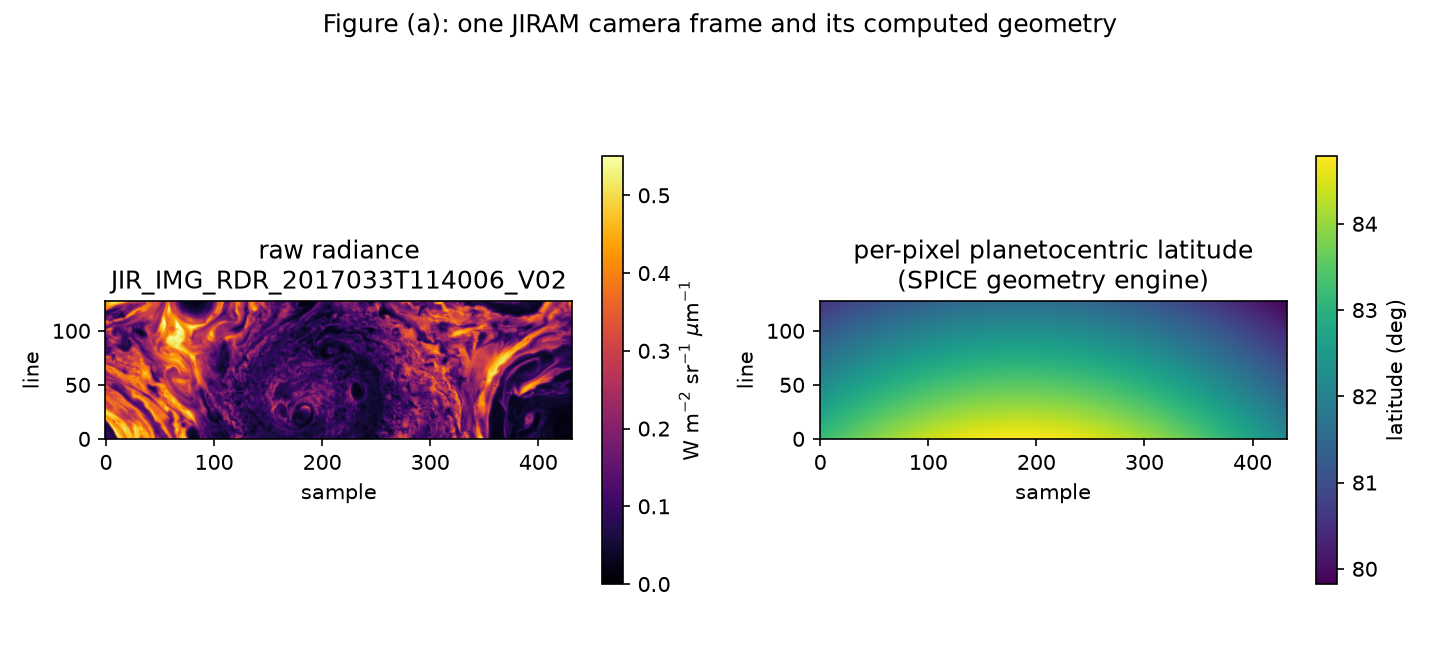
\includegraphics[width=0.95\textwidth]{figures/fig_a_frame_and_latitude.png}
\end{frame}

\begin{frame}{(b) Reproducing a published map from raw bytes}
  \revsec{4.8}
  \centering
  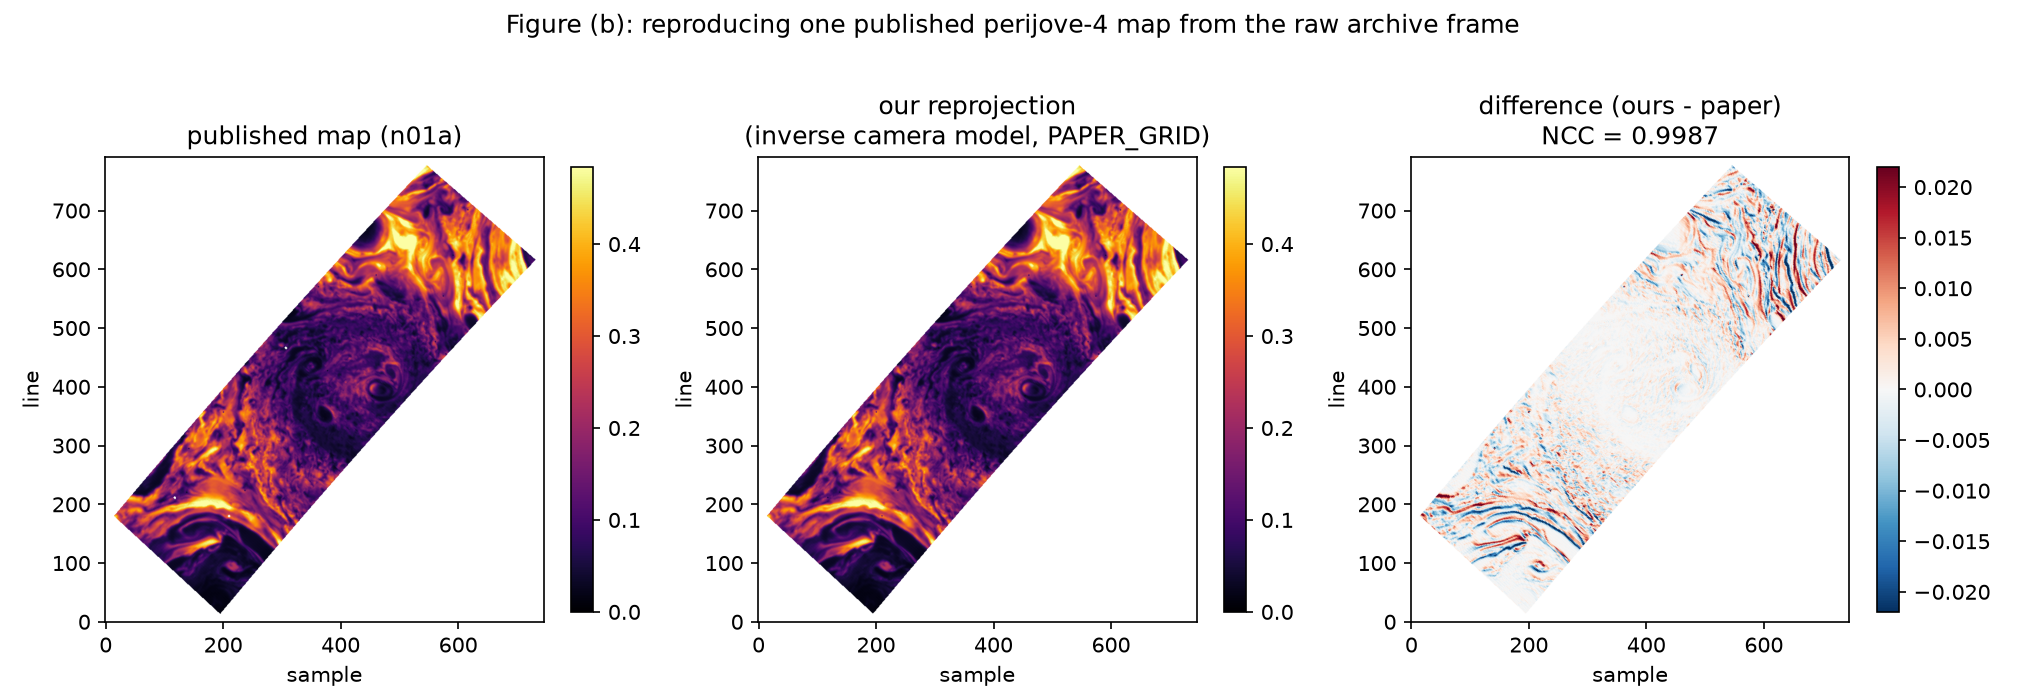
\includegraphics[width=0.98\textwidth]{figures/fig_b_paper_vs_reprojection.png}
\end{frame}

\begin{frame}{(c) A mid-latitude strip, with its graticule}
  \revsec{4.13}
  \centering
  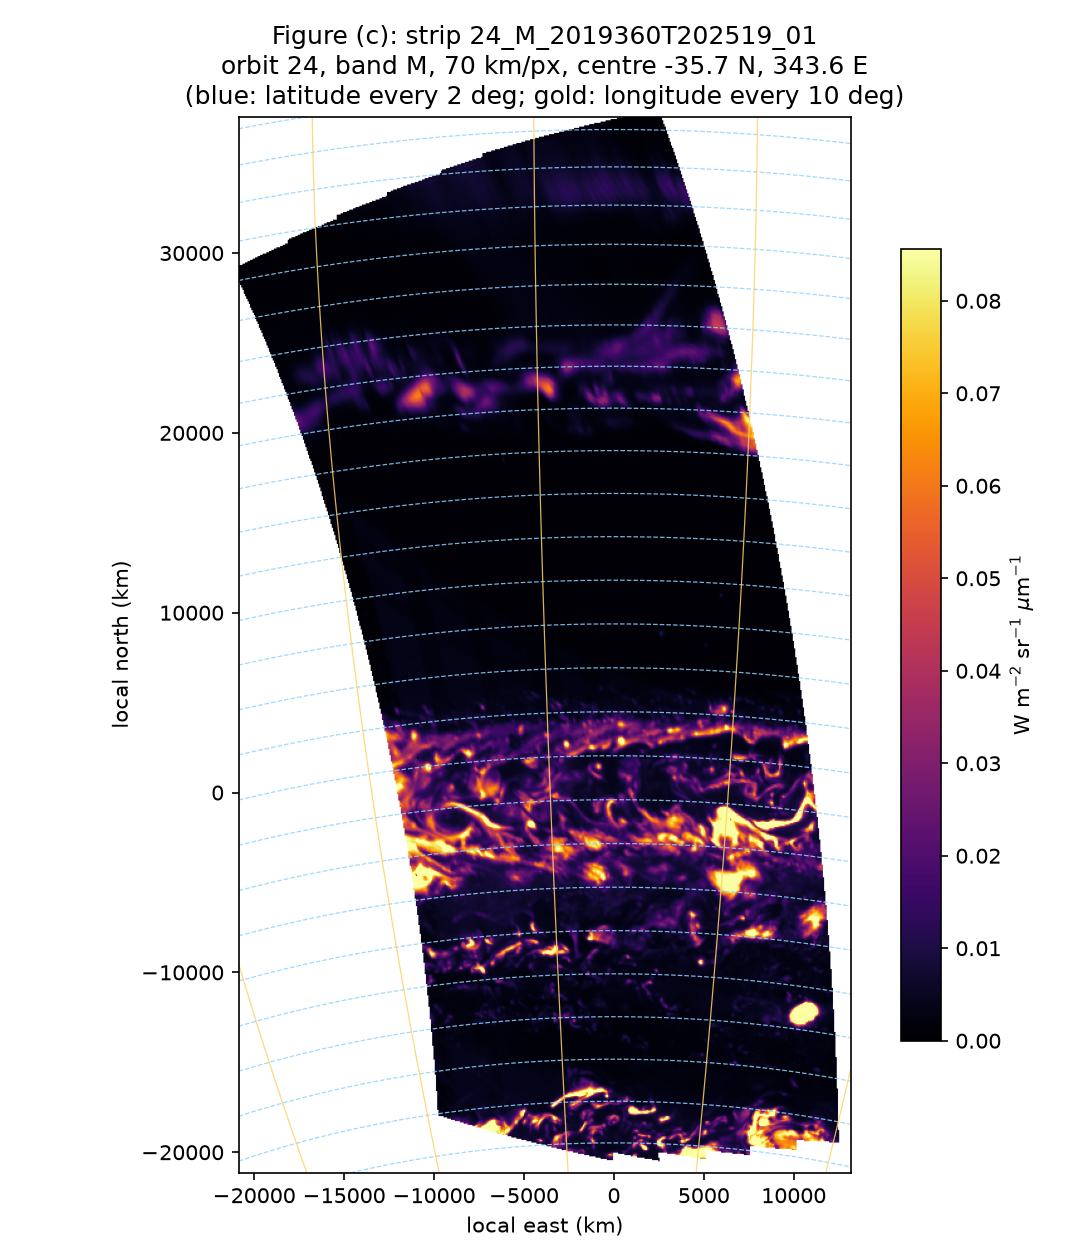
\includegraphics[height=0.82\textheight,keepaspectratio]{figures/fig_c_strip_graticule.png}
\end{frame}

\begin{frame}{(d) That strip's spectrum and structure function}
  \revsec{4.14}
  \centering
  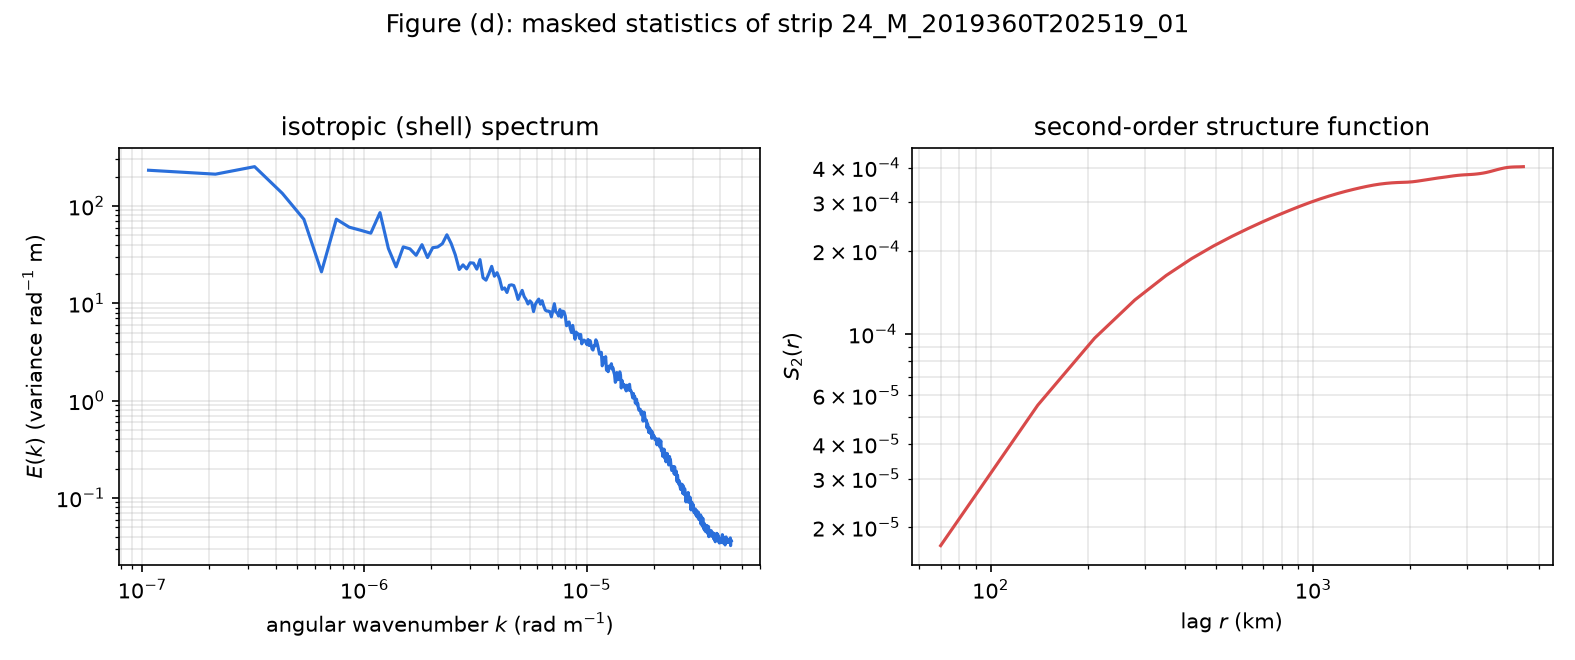
\includegraphics[width=0.95\textwidth]{figures/fig_d_spectrum_structure.png}
\end{frame}

\begin{frame}{(e) The trackability heatmap}
  \revsec{4.15}
  \centering
  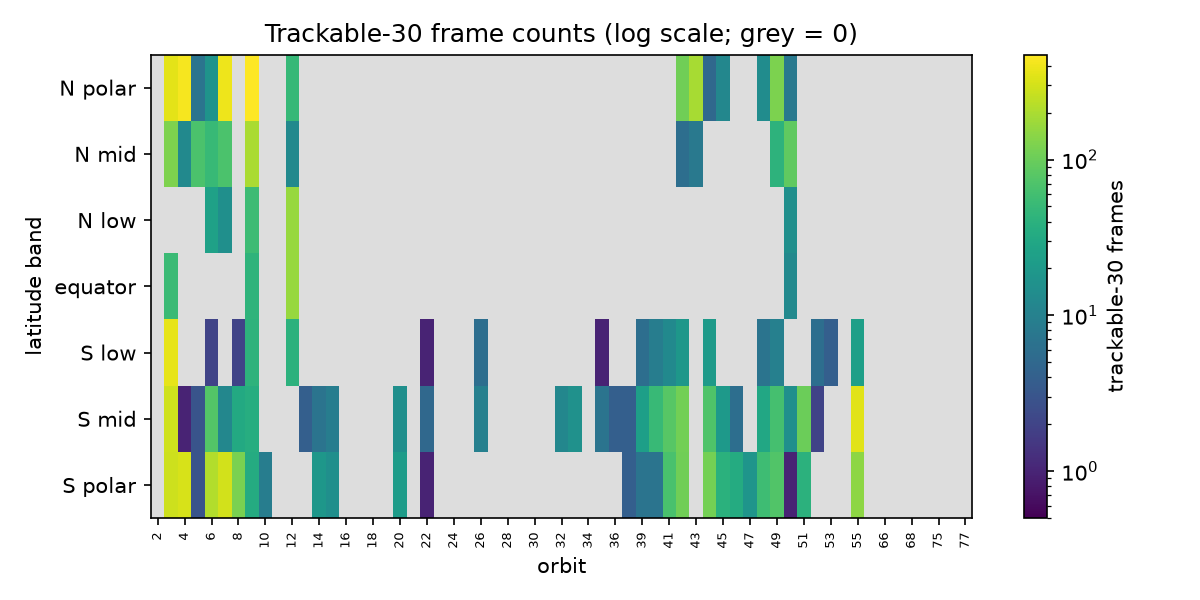
\includegraphics[width=0.88\textwidth]{figures/fig_e_trackability_heatmap.png}
\end{frame}

\begin{frame}{(f) The SPICE frame chain and the pinhole model}
  \revsec{4.4}
  \centering
  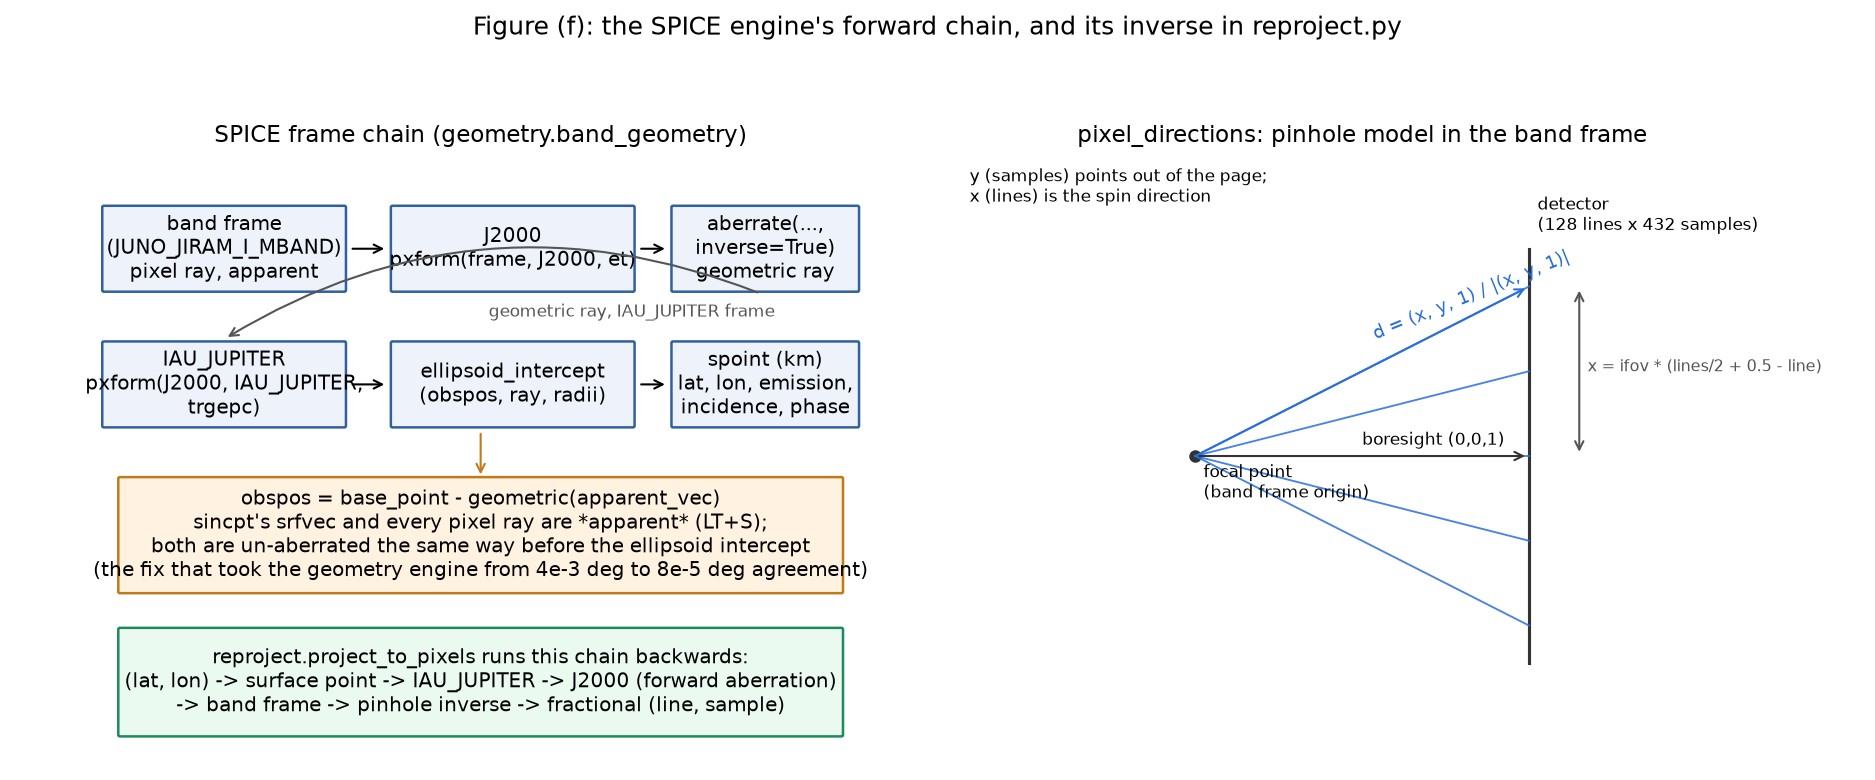
\includegraphics[width=0.98\textwidth]{figures/fig_f_spice_and_pinhole.png}
\end{frame}

% =======================================================================
\section{Testing philosophy}
% =======================================================================

\begin{frame}{Offline tests vs.\ gates}
  \revsec{5}
  \begin{columns}
    \column{0.5\textwidth}
    \textbf{Offline tests}\\
    \small \texttt{test\_*\_offline.py}\\
    no mirror, no network\\
    \texttt{JIRAM\_SKIP\_GATES=1}\\
    synthetic fields, known answers
    \column{0.5\textwidth}
    \textbf{Gates}\\
    \small \texttt{test\_gate\_*.py}\\
    physical gates: real mirror / paper data\\
    contract gates: known synthetic answers\\
    browser gates: complete live interactions
  \end{columns}
  \vspace{0.3cm}
  \textbf{Gates are read-only to every executor, always.} Passing a gate by editing it is task failure --- stated in three separate project documents.
\end{frame}

\begin{frame}{Where acceptance evidence comes from}
  \revsec{5}
  \begin{enumerate}
    \item The 48-frame PJ4 fixture --- numbers a peer-reviewed paper actually published
    \item The published maps and TRACKER4 tables themselves, read directly with \texttt{vicar.py}
    \item A \emph{fresh}, independent SPICE oracle call --- the only kind that can catch a bug in the \emph{vectorisation itself}
    \item Known synthetic shifts, masks, spectra and cadence --- explicit answers for the new workflow contracts; these complement physical validation
  \end{enumerate}
\end{frame}

\begin{frame}{Wrong gate \#1: the geo consistency report}
  \revsec{5}
  All-orbit residuals folded together well-conditioned frames and \emph{partial} (limb) frames, where the label's ``centre'' is a visible-area centroid, not a boresight intercept.
  \begin{quote}\small
    ``geo gate rewritten by lead (well-conditioned median 0.0078 deg; all-orbit report median was inflated by partial/limb frames)''\\
    \hfill---build log, step 8a'
  \end{quote}
  Fix: restrict to fully-on-planet, low-emission frames before computing the statistic.
\end{frame}

\begin{frame}{Wrong gate \#2: the best-baseline definition}
  \revsec{5}
  Original \texttt{best\_dt\_s} rule (``closest to 5~px displacement''): 14/15 gate checks passed on first run --- one failure, from PJ4's dense polar campaign letting a far-in-time sequence coincidentally win.
  \vspace{0.2cm}
  \textbf{Response: investigate, don't loosen the gate.} Redefined to ``smallest $dt$ among trackable partners'' --- no equivalent failure mode; gate tolerance widened to reflect real cadence spread (90~s), not to hide the bug.
\end{frame}

\begin{frame}{The general rule}
  \revsec{5}
  \begin{alertblock}{When a gate fails}
    Investigate why. Never relax the threshold or edit the gate to match whatever the code produced.
  \end{alertblock}
  \vspace{0.2cm}
  \small ``If a threshold is not met, do not tune parameters to pass; investigate ... and report what limits agreement.''\\
  \hfill---\texttt{docs/specs/2026-09-05\_tracking.md}
  \vspace{0.2cm}

  Both wrong-gate stories: the \emph{code} was never the bug --- the gate's own definition was measuring the wrong thing.
\end{frame}

% Refresh through 1e2723d.
\begin{frame}{Validation snapshot: know what each green check proves}
  \revsec{5}
\small At \texttt{1e2723d}, recorded on 7 September 2026:
  \begin{itemize}
    \item 339 offline Python tests passed (49 skipped); 135 frontend unit tests passed
    \item Eight focused live API/policy/science gate checks passed; the full production-bundle browser gate passed
    \item New known answers cover shifts, masks, power laws, cadence, grouping, uncertainty, policy enforcement and out-of-order image responses
    \item The preserved older JunoCam gate has two passes and one count conflict: it expects at least 100 products; current policy admits 72 unique preferred observations
  \end{itemize}
  \vspace{0.2cm}
  The count conflict is reported, not hidden by duplicate versions or weaker exclusions. These checks do not establish archive-wide radiometric or wind accuracy.
\end{frame}

% =======================================================================
\section{How it was built}
% =======================================================================

\begin{frame}{The loop, per milestone}
  \revsec{6}
  \begin{enumerate}
    \item \textbf{Facts first} --- reconnaissance reports numbers, never designs
    \item \textbf{Spec} --- goal, files in scope, every decision explicit, exact validation block
    \item \textbf{Gate before dispatch} --- written by the lead, against ground truth
    \item \textbf{Dispatch} --- one executor, fresh context, the spec is the whole brief
    \item \textbf{Verify} --- scope check, gates run by the lead (not trusted from the report)
    \item \textbf{Record} --- outcome, executor, wall time, gate result $\to$ build log
  \end{enumerate}
  Every spec ends: stop and list ambiguities rather than guess; list every judgment call.
\end{frame}

\begin{frame}{What each executor tier actually did}
  \revsec{6}
  \small
  \begin{itemize}
    \item \textbf{Reconnaissance \& prose:} lighter tier --- 230k tokens settled the two facts the whole design rests on
    \item \textbf{Mechanical code, airtight spec:} cheapest executor that has passed a gate here --- crawler + index, one pass
    \item \textbf{Bounded numerical/geometric work, SPICE/projection oracle, fresh-context review:} stronger tier --- every milestone after the geometry engine, 15--45~min each, 1--3 genuine ambiguities each, resolved sensibly
  \end{itemize}
\end{frame}

\begin{frame}{The stalls, and the ambiguity stops that worked}
  \revsec{6}
  The geometry engine, dispatched three times to the cheaper tier:
  \begin{itemize}
    \item Attempt 1 \& 2: hit a genuine spec ambiguity, \textbf{stopped correctly} --- exactly right
    \item Attempt 3: stalled \textbf{2h12m}, produced nothing --- the failure mode with no automatic detector
  \end{itemize}
  Re-routed to the stronger tier: working engine, aberration fix included, in \textbf{16 minutes}.
  \vspace{0.2cm}
  \textbf{Lesson:} stopping on ambiguity $\neq$ failure. Silent non-progress needs a wall-clock budget, watched by whoever dispatched the work.
\end{frame}

\begin{frame}{Errors executors caught, twice}
  \revsec{6}
  \begin{itemize}
    \item \textbf{Byte order} (little-endian, section 2.2): found \emph{inside} the geometry-augmentation milestone by an executor trusting physical plausibility over the labels; the reprojection gate, written with the documented byte order, failed at the same moment and confirmed it independently
    \item \textbf{Stellar aberration} (section 4.4): a specific, measured 4e-3~deg $\to$ 8e-5~deg fix, found by an executor checking its own output against the same oracle the gate would later check
  \end{itemize}
  Neither was caught by a human re-reading the spec more carefully --- both were caught by checking output against reality.
\end{frame}

\begin{frame}{What this teaches about delegating numerical work}
  \revsec{6}
  \begin{enumerate}
    \item An executor that \textbf{stops on genuine ambiguity} is working correctly --- never penalise this
    \item A gate is only as good as its own definition of ground truth --- distrust a failing gate's assumptions, not just the code under it
    \item Genuine-oracle numerical work (a published number, an independent SPICE call, a known synthetic answer) is exactly where dispatch-then-verify-hard catches real errors --- \emph{in both directions}
  \end{enumerate}
\end{frame}

% Refresh through 1e2723d.
\begin{frame}{The browser revision exposed scientific bugs too}
  \revsec{6}
\begin{itemize}
    \item An apparently harmless version suffix doubled observations and could fabricate cadence; identity belongs in source loaders and exports
    \item A band selector could advance before the pixels arrived; the fix required full request identity and immediate clearing, not a new label
    \item Concurrent NetCDF operations crashed the process; route/job serialization restored correctness while leaving a visible queueing cost
    \item A slow contour path loaded a full large field; bounded display reads improved usability without changing native statistics
  \end{itemize}
  The useful lesson is to test a scientific interaction through its complete source-to-pixel or source-to-export path.
\end{frame}

% =======================================================================
\section{How to extend it}
% =======================================================================

\begin{frame}{Worked example: two extensions, chosen to contrast}
  \revsec{7}
  \begin{enumerate}
    \item A new named region: \texttt{great\_red\_spot} (a \texttt{local\_ortho} patch)
    \item A new statistic: \texttt{skewness} of the radiance field, $\langle(f-\mu)^3\rangle/\sigma^3$
  \end{enumerate}
  \vspace{0.2cm}
  Same loop as every real milestone: facts $\to$ spec $\to$ gate $\to$ module $\to$ wiring $\to$ docs.
\end{frame}

\begin{frame}{Step 1--2: facts, then the spec}
  \revsec{7}
  \textbf{Facts first:} the storm's approximate centre lat/lon at a reference epoch; which orbits actually cover it. For skewness: run it once by hand on a real strip, check the existing \texttt{\_prepare} masking helper is sufficient.
  \vspace{0.2cm}
  \textbf{Spec:} files in scope, a read-only list, the exact API (\texttt{skewness(field, valid=None) -> float}, matching \texttt{structure\_function}'s own calling convention), the validation block.
\end{frame}

\begin{frame}{Step 3: the gate, written first}
  \revsec{7}
  \begin{columns}
    \column{0.5\textwidth}
    \textbf{Region:} no published storm ground truth exists --- gate is \emph{structural}: registry loads, round-trips to 1e-6~px, real-mirror selection is non-empty. Weaker than a scientific gate, and the spec should say so.
    \column{0.5\textwidth}
    \textbf{Statistic:} a \emph{real} numerical gate --- synthetic field with known skewness, tight tolerance, plus a symmetric-field negative control at zero.
  \end{columns}
\end{frame}

\begin{frame}{Step 4--6: module, wiring, docs}
  \revsec{7}
  \begin{itemize}
    \item Region: \textbf{4-line YAML addition} to \texttt{configs/regions.yaml} --- no Python at all
    \item Statistic: \texttt{skewness} added next to \texttt{structure\_function}, reusing \texttt{\_prepare}; one new scalar attr on \texttt{strip\_statistics}'s output
    \item Wiring: region needs none (\texttt{RegionGrid.from\_yaml} is a generic lookup); statistic needs none beyond its own module (already owns its subcommand)
    \item Docs: one line each in \texttt{data\_products.md}, \texttt{architecture.md}, \texttt{open\_items.md} (no ground truth yet)
  \end{itemize}
\end{frame}

\begin{frame}{What the asymmetry teaches}
  \revsec{7}
  \begin{itemize}
    \item Region: almost no code, because \texttt{regions.py} was designed from the start to generalise past its initial four entries
    \item Statistic: real code, but slotted directly into an existing, well-established pattern --- no new architecture needed
  \end{itemize}
  \vspace{0.3cm}
  Neither extension needed a new pattern invented on the spot --- that is itself a finding about the codebase, not just a tutorial.
\end{frame}

% =======================================================================
\section{Glossary}
% =======================================================================

\begin{frame}{Glossary: SPICE}
  \revsec{8}
  \scriptsize
  \begin{itemize}
    \item \textbf{SPICE}: NAIF's toolkit for spacecraft geometry from loaded \emph{kernels}
    \item \textbf{Kernel} (SPK/CK/FK/IK/SCLK/LSK/PCK): trajectory / attitude / frames / instrument / clock / leap-seconds / planetary-constants files
    \item \textbf{Furnsh / kernel pool}: SPICE state is global per process --- why every parallel worker here uses \texttt{spawn}, never \texttt{fork}
    \item \textbf{Ephemeris time (ET)}: SPICE time scale. JIRAM uses label start time; JunoCam adds instrument timing terms per frame and any fitted offset
    \item \textbf{Sincpt} / \textbf{pxform}: surface-intercept and frame-rotation calls; \texttt{geometry.py} vectorises the same computation over a whole pixel grid
    \item \textbf{Light time / stellar aberration (``LT+S'')}: finite light speed, and the observer's own velocity bending apparent direction --- getting the \emph{inverse} applied consistently is section 4.4's central subtlety
  \end{itemize}
\end{frame}

\begin{frame}{Glossary: geometry conventions}
  \revsec{8}
  \scriptsize
  \begin{itemize}
    \item \textbf{Planetocentric} latitude: angle from the equatorial plane to the vector from the body's \emph{centre} --- the convention of native repository grids
    \item \textbf{Planetographic} latitude: uses the local surface normal instead --- different on an oblate body; the external ML-calibrated reference requires conversion
    \item \textbf{East-positive longitude, [0,360)}: this project's fixed convention, matching the archive's own labels
    \item \textbf{System III}: Jupiter's body-fixed rotating longitude system; \texttt{IAU\_JUPITER} \emph{is} System III for this project's purposes
    \item \textbf{Emission / incidence / phase angle}: angle to observer / to Sun / between the two, at the surface point
    \item \textbf{Orthographic / stereographic / equidistant / Lambert}: four radial laws relating map distance to true angular distance; the published maps use orthographic, despite the literature calling them stereographic
  \end{itemize}
\end{frame}

\begin{frame}{Glossary: archive \& this codebase}
  \revsec{8}
  \scriptsize
  \begin{itemize}
    \item \textbf{PDS3 / PDS4}: the archive's label syntax (PDS3 text) and bundle layout (PDS4 directories) --- not the same axis
    \item \textbf{RDR / EDR}: reduced / experimental data record. Processing level alone does not establish units: JIRAM RDR is radiance; native JunoCam remains DN
    \item \textbf{VICAR}: JPL's older self-contained image format --- used here only because the ground-truth maps and vector tables ship in it
    \item \textbf{NCC}: normalised cross-correlation, 1.0 for identical patches --- the tracker's match score \emph{and} the general ``does our reprojection match the paper'' figure of merit
    \item \textbf{\texttt{geo\_ok} / \texttt{on\_planet\_frac} / \texttt{bore\_*}}: SPICE succeeded at all / fraction of pixels on the ellipsoid / evaluated at the boresight specifically --- consistent naming across every table in this codebase
  \end{itemize}
\end{frame}

% Refresh through 1e2723d.
\begin{frame}{Glossary: the new scientific contracts}
  \revsec{8}
\small
  \begin{itemize}
    \item \textbf{Framelet}: one filter strip's 128-line readout; many framelets make one JunoCam archived image
    \item \textbf{Observation identity}: the underlying exposure identity, independent of processing-version suffix
    \item \textbf{Eligibility}: evidence-based access under the current policy; distinct from absolute radiometric calibration
    \item \textbf{Readiness}: format, grid, cadence and mask compatibility for an operation; distinct from physical accuracy
    \item \textbf{Normalization / stretch}: transformation of the analysed field / mapping to display brightness
    \item \textbf{Independent pass}: the population uncertainty unit; overlapping strips are not independent replicates
  \end{itemize}
\end{frame}

\begin{frame}[plain]
  \revsec{}
  \centering
  \vspace{1.5cm}
  {\LARGE\color{jirblue}\textbf{Where to read next}}
  \vspace{0.6cm}

  \begin{tabular}{ll}
    full detail & \texttt{PEDAGOGICAL\_REVIEW.md} \\
    module-by-module facts & \texttt{docs/architecture.md}, \texttt{docs/decisions.md} \\
    schemas & \texttt{docs/data\_products.md} \\
    command reference & \texttt{docs/usage.md} \\
    current browser/science use & \texttt{docs/research\_workflow.md} \\
    open questions & \texttt{docs/open\_items.md} \\
  \end{tabular}\par
  \vspace{1cm}

  {\small\color{jirgray} This deck and its figures: \texttt{docs/pedagogy/}}
\end{frame}

\end{document}
